
% === Pali ===

\cleartoverso

\vspace*{30mm}

\begin{verse}

\verseref{1}
\emph{pucchāmi taṁ ādiccabandhu\\
vivekaṁ santipadañca mahesi}\\
\emph{kathaṁ disvā nibbāti bhikkhu\\
anupādiyāno lokasmiṁ kiñci}

\verseref{2}
mūlaṁ papañcasaṅkhāya\\
mantā asmīti sabbamuparundhe\\
yā kāci taṇhā ajjhattaṁ\\
tāsaṁ vinayā sadā sato sikkhe

\verseref{3}
yaṁ kiñci dhammamabhijaññā\\
ajjhattaṁ atha vāpi bahiddhā\\
na tena thāmaṁ kubbetha\\
na hi sā nibbuti sataṁ vuttā

\verseref{4}
seyyo na tena maññeyya\\
nīceyyo athavāpi sarikkho\\
phuṭṭho anekarūpehi\\
nātumānaṁ vikappayaṁ tiṭṭhe

\verseref{5}
ajjhattamevupasame\\
na aññato bhikkhu santimeseyya\\
ajjhattaṁ upasantassa\\
natthi attā kuto nirattā vā

\verseref{6}
majjhe yathā samuddassa\\
ūmi no jāyatī ṭhito hoti\\
evaṁ ṭhito anejassa\\
ussadaṁ bhikkhu na kareyya kuhiñci

\verseref{7}
\emph{akittayī vivaṭacakkhu\\
sakkhidhammaṁ parissayavinayaṁ}\\
\emph{paṭipadaṁ vadehi bhaddante\\
pātimokkhaṁ atha vāpi samādhiṁ}

\verseref{8}
cakkhūhi neva lolassa\\
gāmakathāya āvaraye sotaṁ\\
rase ca nānugijjheyya\\
na ca mamāyetha kiñci lokasmiṁ

\verseref{9}
phassena yadā phuṭṭhassa\\
paridevaṁ bhikkhu na kareyya kuhiñci\\
bhavañca nābhijappeyya\\
bheravesu ca na sampavedheyya

\verseref{10}
annānamatho pānānaṁ\\
khādanīyānaṁ athopi vatthānaṁ\\
laddhā na sannidhiṁ kayirā\\
na ca parittase tāni alabhamāno

\verseref{11}
jhāyī na pādalolassa\\
virame kukkuccā nappamajjeyya\\
athāsanesu sayanesu\\
appasaddesu bhikkhu vihareyya

\verseref{12}
niddaṁ na bahulīkareyya\\
jāgariyaṁ bhajeyya ātāpī\\
tandiṁ māyaṁ hassaṁ khiḍḍaṁ\\
methunaṁ vippajahe savibhūsaṁ

\verseref{13}
āthabbaṇaṁ supinaṁ lakkhaṇaṁ\\
no vidahe athopi nakkhattaṁ\\
virutañca gabbhakaraṇaṁ\\
tikicchaṁ māmako na seveyya

\verseref{14}
nindāya nappavedheyya\\
na uṇṇameyya pasaṁsito bhikkhu\\
lobhaṁ saha macchariyena\\
kodhaṁ pesuṇiyañca panudeyya

\verseref{15}
kayavikkaye na tiṭṭheyya\\
upavādaṁ bhikkhu na kareyya kuhiñci\\
gāme ca nābhisajjeyya\\
lābhakamyā janaṁ na lapayeyya

\verseref{16}
na ca katthitā siyā bhikkhu\\
na ca vācaṁ payuttaṁ bhāseyya\\
pāgabbhiyaṁ na sikkheyya\\
kathaṁ viggāhikaṁ na kathayeyya

\verseref{17}
mosavajje na nīyetha\\
sampajāno saṭhāni na kayirā\\
atha jīvitena paññāya\\
sīlabbatena nāññamatimaññe

\verseref{18}
sutvā rusito bahuṁ vācaṁ\\
samaṇānaṁ vā puthujanānaṁ\\
pharusena ne na paṭivajjā\\
na hi santo paṭisenikaronti

\verseref{19}
etañca dhammamaññāya\\
vicinaṁ bhikkhu sadā sato sikkhe\\
santīti nibbutiṁ ñatvā\\
sāsane gotamassa na pamajjeyya

\verseref{20}
abhibhū hi so anabhibhūto\\
sakkhidhammamanītihamadassī\\
tasmā hi tassa bhagavato sāsane\\
appamatto sadā namassamanusikkheti

\end{verse}

% === Slovenian ===

\chapter[Tuvaṭaka Sutta]{{kama-sutta-gray.png}{ucenje-2.png}}

% Učenje o hitrosti

\begin{verse}

%\vFirst
%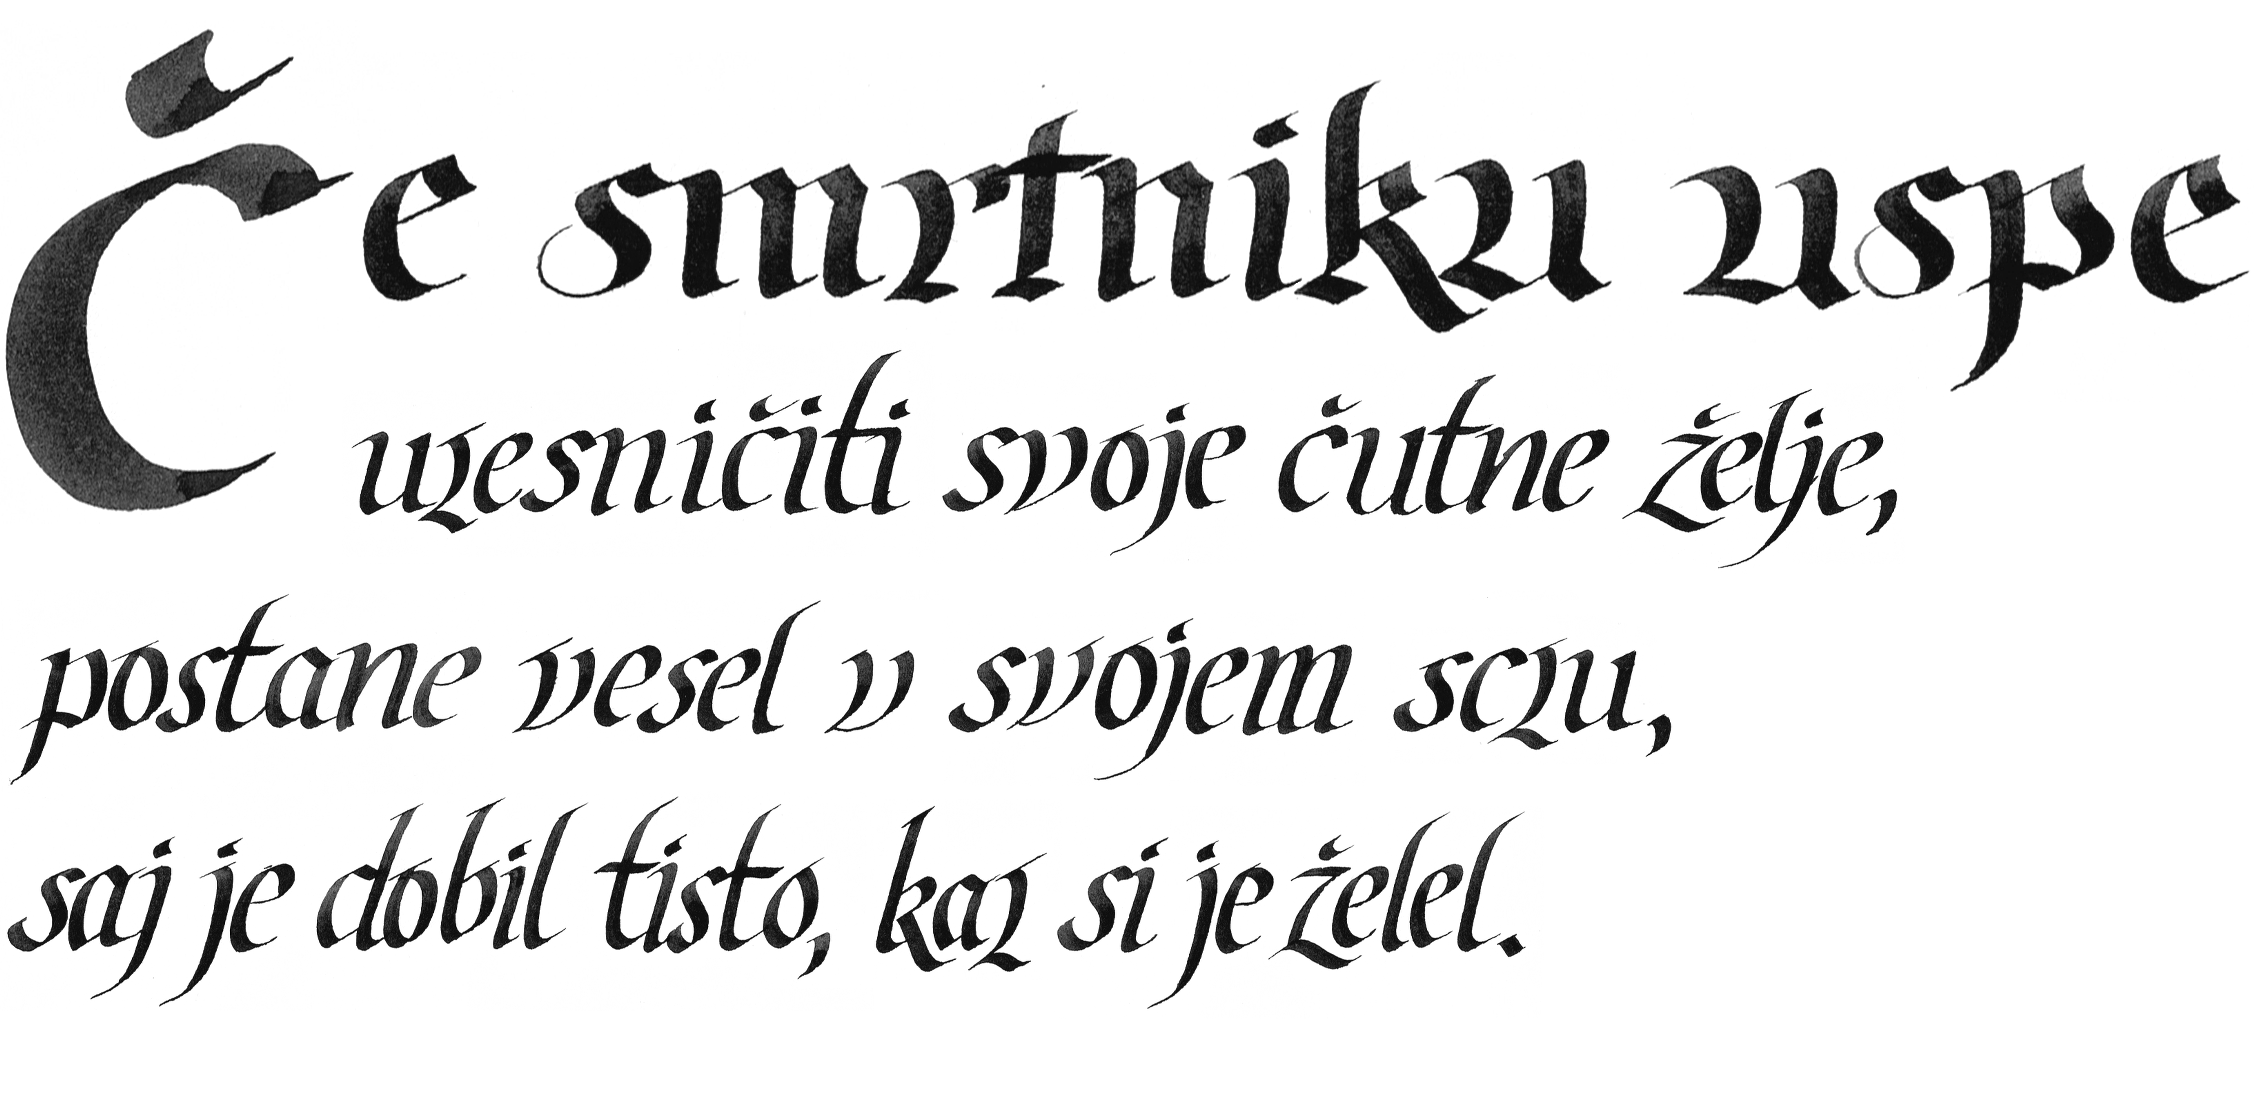
\includegraphics[scale=0.3]{ce-smrtniku-gray.png}

\verseref{1}
\emph{Sprašujem sorodnika sonca,}\\
\emph{Njegovo svetost, o samoti in o stanju miru:}\\
\emph{s kakšnim védenjem je lahko menih ugasnjen,}\\
\emph{da se ne bi vezal na nič v tem svetu?}

\verseref{2}
Popolnoma naj bi prenehal misliti: »Jaz sem«,\\
to celotno korenino uveljavljene obsedenosti.\\
Ne glede koliko hrepenenja je še v njem,\\
bo v popolni pozornosti vadil to razrešitev.

\verseref{3}
Katerekoli ideje, ki jih pozna,\\
ne glede če te izvirajo od znotraj ali prihajajo od zunaj,\\
z njimi si ne bo utrjeval stališča,\\
saj krepostni tega ne bi imenovali »mir«.

\verseref{4}
Ne bo se imel za boljšega,\\
ne za slabšega niti ne za enakovrednega.\\
Čeprav dotaknjen z mnogimi stvarmi,\\
ne bo zagovarjal misli o sebi.

\verseref{5}
Le v sebi lahko pride do miru,\\
menih ga ne bo iskal v zunanjem svetu.\\
Za tistega, ki je v miru sam s seboj,\\
ni ničesar za pridobiti, kaj šele za zavreči.

\verseref{6}
Tako, kot je sredi morja\\
popolnoma mirno in ni nobenih valov,\\
tako tudi brez hrepenenja človek mirno biva --\\
tak menih si ne bo jemal časti.

\verseref{7}
\emph{Čigar oči so odprte z odloženimi težavami,}\\
\emph{ta je razložil Dhammo, kot jo je sam spoznal.}\\
\emph{Častiti gospod, povejte nam o poteku napredka,}\\
\emph{o etični dolžnosti in tudi o koncentraciji.}

\verseref{8}
Menih ne dovoli, da so njegove oči nemirne,\\
svoja ušesa zapre pred vaškimi govoricami,\\
ni požrešen na okuse\\
in ničesar v svetu ne jemlje, kot »to je moje«.

\verseref{9}
Kadarkoli je menih v stiku z neprijetnostmi,\\
se ne predaja žalovanju.\\
Ne hrepeni po obstoju,\\
niti ni pretresen zaradi strahu.

\verseref{10}
Hrano in pijačo,\\
živila in tudi oblačila --\\
vsa ta imetja ne bo imel za zaklad\\
niti se ne bo bal njihovega pomanjkanja.

\verseref{11}
Meditant, ki se brez želja po tavanju naokrog\\
vzdrži obžalovanih dejanj, je pazljiv.\\
Kjerkoli ima namen sedeti ali ležati,\\
menih naj živi v kraju z malo motenj.

\verseref{12}
Naj ne spi predolgo,\\
marljiv v opreznosti naj vztraja v budnosti.\\
Tako bo zapustil vse: lenobo, iluzije, smeh, igre,\\
spolnost in vse njihove izpeljanke.

\verseref{13}
Ritualno zdravljenje naj ne bo njegova praksa,\\
niti ne razlaga sanj, tolmačenje znakov in astrologije.\\
Učenec ne bo tolmačil živalskih krikov,\\
zdravil neplodnost ali druge bolezni.

\verseref{14}
Menih naj ne bo pretresen zaradi kritik,\\
niti ne vzvišen zaradi pohval.\\
Pregnal bo celotno hrepenenje,\\
skupaj s strahom pred izgubo, jezo in žalitve.

\verseref{15}
Menih naj ne kupuje in ne prodaja,\\
nobenih kritik naj ne raznaša,\\
naj ne bo nadloga med ljudmi\\
in laskajoč z željami po koristi.

\verseref{16}
Menih naj se ne hvali,\\
niti naj ne izreka besed s skritimi motivi,\\
naj ne vadi v predrznem obnašanju,\\
in naj se izogne govorom o spornih temah.

\verseref{17}
Naj se ne predaja lažem;\\
tako s popolno pozornostjo ne bo zlorabljal zaupanja.\\
Hkrati naj nobenega ne prezira\\
zaradi njegovega življenja, razumevanja, morale ali običajev.

\verseref{18}
Ko sliši mnogo besed in je izzvan\\
od mislecev in nevednih ljudi,\\
nazaj naj jim ne odgovarja ostro,\\
saj si tisti z vrlinami ne dela sovražnikov.

\verseref{19}
Menih bo s takim razumevanjem Dhamme,\\
vadil v skladu s proučevanjem, s pozornostjo\\
in z razumevanjem stanja prenehanja kot miru,\\
tako ne bo zanemarjal Gotamovega učenja.

\verseref{20}
On je resnično osvajalec neosvojenega,\\
uvidel je resnico, ki temelji na izkušnji in ne na govoricah.\\
Zato se vedno spoštljivo pokloni\\
in pazljivo vadi po vodilu Blaženega.


\end{verse}

% === Pali ===

\clearpage
\begin{verse}

\verseref{5}

\end{verse}

% === Slovenian ===

\clearpage
\begin{verse}

\verseref{5}

\end{verse}

